\chapter{Implementación, Pruebas y Resultados}

\section{Descripción de la Solución}
El prototipo entrega cuatro productos: (1) el pipeline de datos y modelado, (2) los artefactos del modelo, (3) una API REST y (4) un tablero web (Figura~\ref{fig:arquitectura}). La Tabla~\ref{tab:stack} indica las tecnologías y versiones empleadas; el detalle técnico está en el Anexo~A y el manual de uso en el Anexo~B.

\begin{table}[H]
  \caption{Tecnologías empleadas y versiones.}
  \label{tab:stack}
  \tablabase\footnotesize
  \begin{tabular}{|p{3.0cm}|p{3.2cm}|p{2.2cm}|p{4.4cm}|}
    \hline
    \enc{Componente} & \enc{Tecnología} & \enc{Versión} & \enc{Uso}\\ \hline
    Modelado & scikit-learn & 1.6.1 & Pipeline, comparación y búsqueda de hiperparámetros\\ \hline
    Modelado & XGBoost & 2.1.4 & Algoritmo candidato\\ \hline
    Datos & pandas / numpy & $\geq$ 2.2.3 / $\geq$ 2.1.0 & Carga y transformación\\ \hline
    Serialización & joblib & 1.5.1 & Guardado del \textit{Pipeline} completo\\ \hline
    Servicio web & FastAPI / Uvicorn & 0.116.1 / 0.35.0 & API REST\\ \hline
    Exportación & openpyxl & 3.1.5 & Resultados masivos en \texttt{.xlsx}\\ \hline
    Tablero & React / Vite & 19 / --- & Interfaz web\\ \hline
    Despliegue & Render (API) / Vercel (tablero) & --- & Publicación del prototipo\\ \hline
  \end{tabular}
\end{table}

\section{Proceso de Implementación}
\subsection{Preparación de los datos}
El pipeline parte de los \num{20510} registros y 350 variables del módulo de salud de la niñez. Se normalizaron los nombres de las variables, se convirtieron los valores especiales en nulos y se conservaron 114 predictores (Tabla~\ref{tab:vars}). Se excluyeron los \num{2017} registros sin variable objetivo, con lo que la base final quedó en \num{18493} registros. La base original tenía valores ausentes en 84 de los 114 predictores (en 32 superaban el \SI{10}{\percent}; por ejemplo, \SI{56.1}{\percent} en el peso al nacer, \SI{57.3}{\percent} en la talla al nacer y \SI{62.8}{\percent} en el perímetro cefálico). La base del modelo, en cambio, no contiene nulos: los faltantes se imputaron con mediana o moda en la limpieza inicial, sobre todos los registros y antes de la partición entrenamiento/prueba. El notebook original de esa limpieza se recuperó del historial del repositorio y confirma el procedimiento: moda para variables categóricas y mediana para numéricas, sobre la base completa (Anexo~G).

\subsection{Corrección de la versión inicial}
La primera versión del modelo (v1) imputaba con la mediana la propia variable objetivo faltante, lo que creaba \num{2017} etiquetas inexistentes, todas de la clase 0. Además, elegía el modelo ganador por F1 ponderado pero optimizaba siempre XGBoost, y publicaba métricas fijas en la API que no se reproducían. Estas fallas se detectaron en una revisión del pipeline y se corrigieron en una segunda versión (v2), que es la que se reporta en este documento. Al reevaluar la v1 con su propia partición se obtuvo exactitud de 0.655, sensibilidad de 0.476 y ROC-AUC de 0.648. La Tabla~\ref{tab:v1v2} resume las diferencias.

\begin{table}[H]
  \caption{Diferencias entre la versión inicial (v1) y la corregida (v2).}
  \label{tab:v1v2}
  \tablabase\footnotesize
  \begin{tabular}{|p{3.2cm}|p{4.8cm}|p{5.2cm}|}
    \hline
    \enc{Aspecto} & \enc{v1 (descartada)} & \enc{v2 (reportada)}\\ \hline
    Variable objetivo faltante & Imputada con la mediana (\num{2017} registros) & Registros excluidos\\ \hline
    Selección del modelo & Se optimizaba XGBoost sin importar el ganador & Selección real por PR-AUC entre cuatro modelos\\ \hline
    Desbalance & Sin tratamiento & Ponderación de clases y ajuste del umbral\\ \hline
    Métricas principales & Promedios ponderados (exactitud, F1 ponderado) & Métricas por clase, ROC-AUC y PR-AUC\\ \hline
    Métricas de la API & Valores fijos en el código & Leídas de \texttt{metricas\_v2.json}\\ \hline
  \end{tabular}
\end{table}

\subsection{Exploración y control de fuga}
La exploración comparó la prevalencia en Tungurahua y en el conjunto nacional (Figura~\ref{fig:prevalencia}). Para controlar la fuga se hizo un examen univariado: ninguna variable, por sí sola, discrimina la variable objetivo con AUC superior a 0.95. También se revisó el listado de predictores: no incluye talla ni peso actuales del niño. Persisten dos variables de diseño muestral, \texttt{factor\_expansion} y \texttt{estrato}, que no describen al niño y cuya presencia se trata como limitación. Como el imputador del \textit{Pipeline} no tiene efecto (la base ya no tiene nulos), la imputación previa a la partición constituye una fuga leve de información desde la prueba hacia el entrenamiento, cuyo efecto no se cuantificó.

\subsection{Modelado y protocolo experimental}
La Tabla~\ref{tab:experimento} reúne el experimento en una sola vista, y la Figura~\ref{fig:comparacion} compara los cuatro modelos base. Random Forest obtuvo el mayor PR-AUC (0.411), seguido de la regresión logística (0.391), XGBoost (0.368) y el árbol de decisión (0.263); la prevalencia (0.247) es el nivel de referencia de un clasificador sin información. Tras ajustar hiperparámetros con regularización, el PR-AUC del modelo final fue 0.409, sin mejora frente al modelo base, pero con menor sobreajuste y menor tamaño.

\begin{table}[H]
  \caption{Tabla única del experimento.}
  \label{tab:experimento}
  \tablabase\footnotesize
  \begin{tabular}{|p{3.2cm}|p{10.2cm}|}
    \hline
    \enc{Aspecto} & \enc{Valor}\\ \hline
    Dataset & ENSANUT 2018 (Ecuador), módulo de salud de la niñez\\ \hline
    Muestra final & \num{18493} registros (se excluyeron \num{2017} sin variable objetivo)\\ \hline
    Variable objetivo & \texttt{desnutricion\_cronica} (0 = sin, 1 = con); \SI{24.7}{\percent} de clase 1\\ \hline
    Predictores & 114 variables\\ \hline
    Partición & 80/20 estratificada, semilla 42: \num{14794} entrenamiento y \num{3699} prueba\\ \hline
    Preprocesamiento & Numéricas: estandarización. Categóricas: \textit{one-hot}. Imputación (mediana o moda) ya aplicada antes de la partición\\ \hline
    Modelos comparados & Regresión logística, árbol de decisión, Random Forest y XGBoost, con manejo de desbalance\\ \hline
    Criterio de selección & PR-AUC (\textit{average precision}), no F1 ponderado\\ \hline
    Modelo ganador & Random Forest: 300 árboles, profundidad máxima 20, mínimo 10 muestras por hoja, \texttt{max\_features="sqrt"}, \texttt{class\_weight="balanced"}\\ \hline
    Búsqueda de hiperparámetros & \textit{RandomizedSearchCV}, validación cruzada estratificada de 5 particiones, criterio PR-AUC\\ \hline
    Umbral de decisión & 0.42 (maximiza el F1 de la clase 1 con validación cruzada sobre el entrenamiento)\\ \hline
  \end{tabular}
\end{table}

\begin{figure}[H]
  \centering
  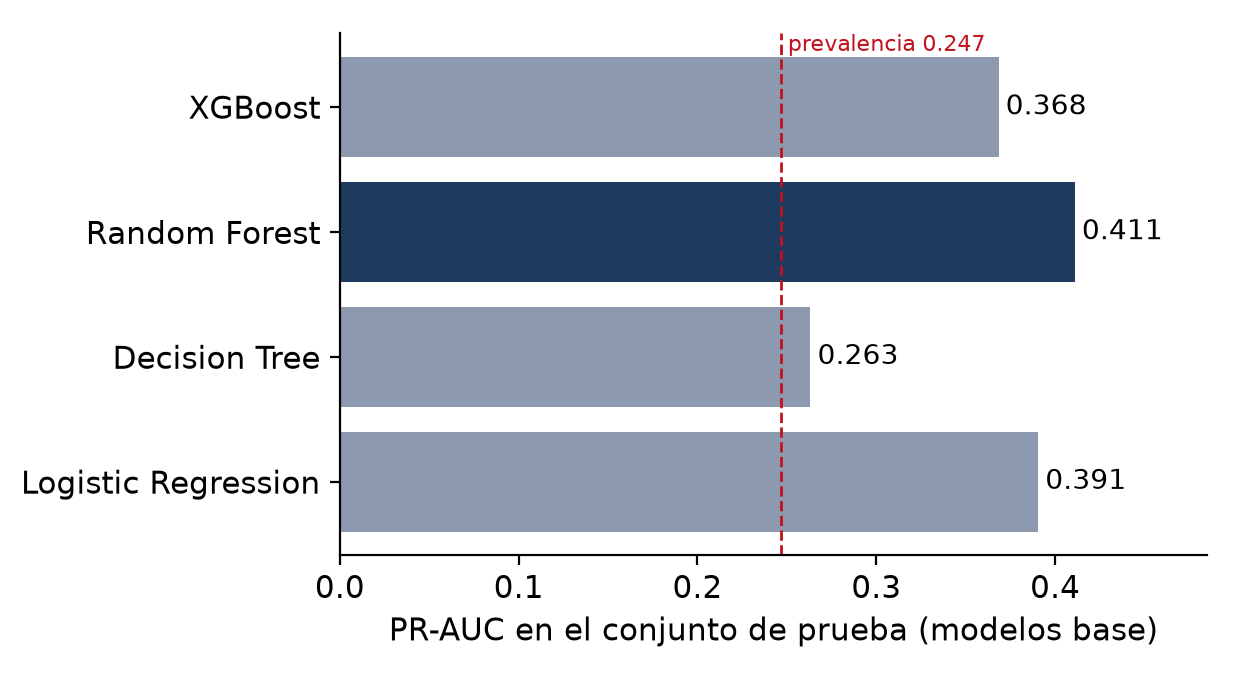
\includegraphics[width=0.7\textwidth]{figuras/comparacion-modelos.png}
  \caption{Comparación de los cuatro modelos base por PR-AUC en el conjunto de prueba. Elaboración propia.}
  \label{fig:comparacion}
\end{figure}

\subsection{API y tablero}
La API carga el \textit{Pipeline} serializado, valida que la solicitud contenga exactamente las 114 variables y devuelve la clase, la probabilidad y un nivel de riesgo. La clase se asigna con el umbral de 0.42. El tablero en React consume la API para mostrar indicadores, métricas y los módulos de clasificación individual y por archivo (Anexo~B). Su interfaz se revisó y corrigió durante la elaboración de este documento (cambios publicados en el repositorio, Anexo~E).

\section{Pruebas y Validación}
Se realizaron dos tipos de pruebas, que evalúan aspectos distintos y no deben confundirse:
\begin{itemize}
  \item \textbf{Evaluación del modelo:} desempeño predictivo sobre la partición de prueba (interna) y sobre su subconjunto de Tungurahua. No es una validación externa, porque la partición proviene de la misma encuesta y el mismo protocolo.
  \item \textbf{Pruebas funcionales de la API:} verifican que el servicio responda según su contrato. Un resultado favorable indica que el software funciona, no que la predicción sea válida clínicamente.
\end{itemize}

Las pruebas funcionales incluyeron 17 casos (Anexo~C) y las 21 pruebas automáticas del repositorio. Las 21 pruebas y 16 de los 17 casos se cumplieron; falló CP15 (la puntuación del formulario individual casi no varía con los datos). CP14 (archivo Excel enviado directamente a la API) falló en la versión evaluada inicialmente y se volvió a ejecutar con el servicio corregido (Anexo~C). La latencia de \texttt{POST /predict}, medida en 100 solicitudes en ejecución local (sin red), tuvo mediana de 29 ms, percentil 95 de 33 ms y máximo de 38 ms. Como comprobación de consistencia, la probabilidad devuelta por la API para un registro coincidió con la calculada directamente sobre el modelo (0.437).

\section{Resultados}
\subsection{Desempeño en el conjunto de prueba nacional}
La Tabla~\ref{tab:metricas} presenta las métricas con el umbral de 0.42, con intervalos de confianza del \SI{95}{\percent} obtenidos por \textit{bootstrap} (1000 remuestreos). La Figura~\ref{fig:matriz} muestra la matriz de confusión y la Figura~\ref{fig:curvas} las curvas ROC y de precisión--sensibilidad.

De los 912 niños con desnutrición crónica del conjunto de prueba, el modelo identificó 632 (sensibilidad de 0.693). A cambio, clasificó como positivos a \num{1255} de los \num{2787} niños sin desnutrición (especificidad de 0.550), por lo que solo una de cada tres alertas es un caso real (precisión de 0.335, frente a una prevalencia de 0.247). El ROC-AUC de 0.677 indica una capacidad de discriminación moderada.

\begin{table}[H]
  \caption{Métricas del modelo en el conjunto de prueba nacional ($n$~=~\num{3699}, umbral 0.42).}
  \label{tab:metricas}
  \tablabase\small
  \begin{tabular}{|p{5.6cm}|c|c|}
    \hline
    \enc{Métrica} & \enc{Valor} & \enc{IC 95\,\%}\\ \hline
    Sensibilidad (clase 1) & 0.693 & 0.664--0.723\\ \hline
    Especificidad (clase 0) & 0.550 & ---\\ \hline
    Precisión (clase 1) & 0.335 & ---\\ \hline
    F1 (clase 1) & 0.452 & 0.429--0.473\\ \hline
    Exactitud balanceada & 0.621 & ---\\ \hline
    ROC-AUC & 0.677 & 0.657--0.696\\ \hline
    PR-AUC (referencia: 0.247) & 0.409 & 0.377--0.442\\ \hline
  \end{tabular}
\end{table}

\begin{figure}[H]
  \centering
  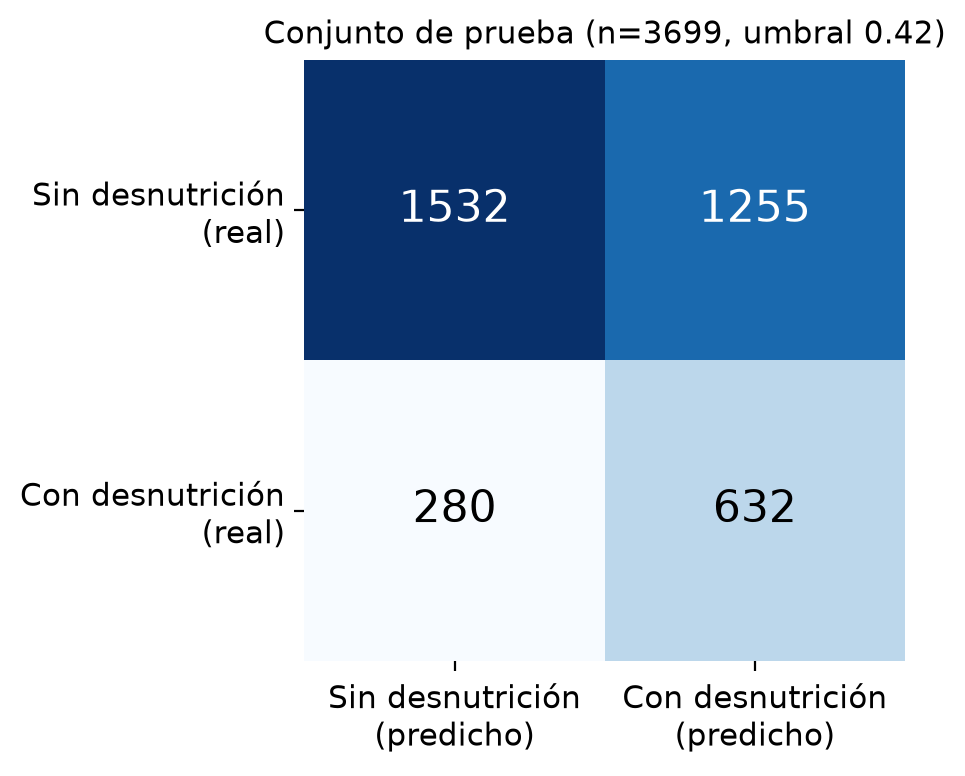
\includegraphics[width=0.55\textwidth]{figuras/matriz-confusion-global.png}
  \caption{Matriz de confusión en el conjunto de prueba nacional (umbral 0.42). Elaboración propia.}
  \label{fig:matriz}
\end{figure}

\begin{figure}[H]
  \centering
  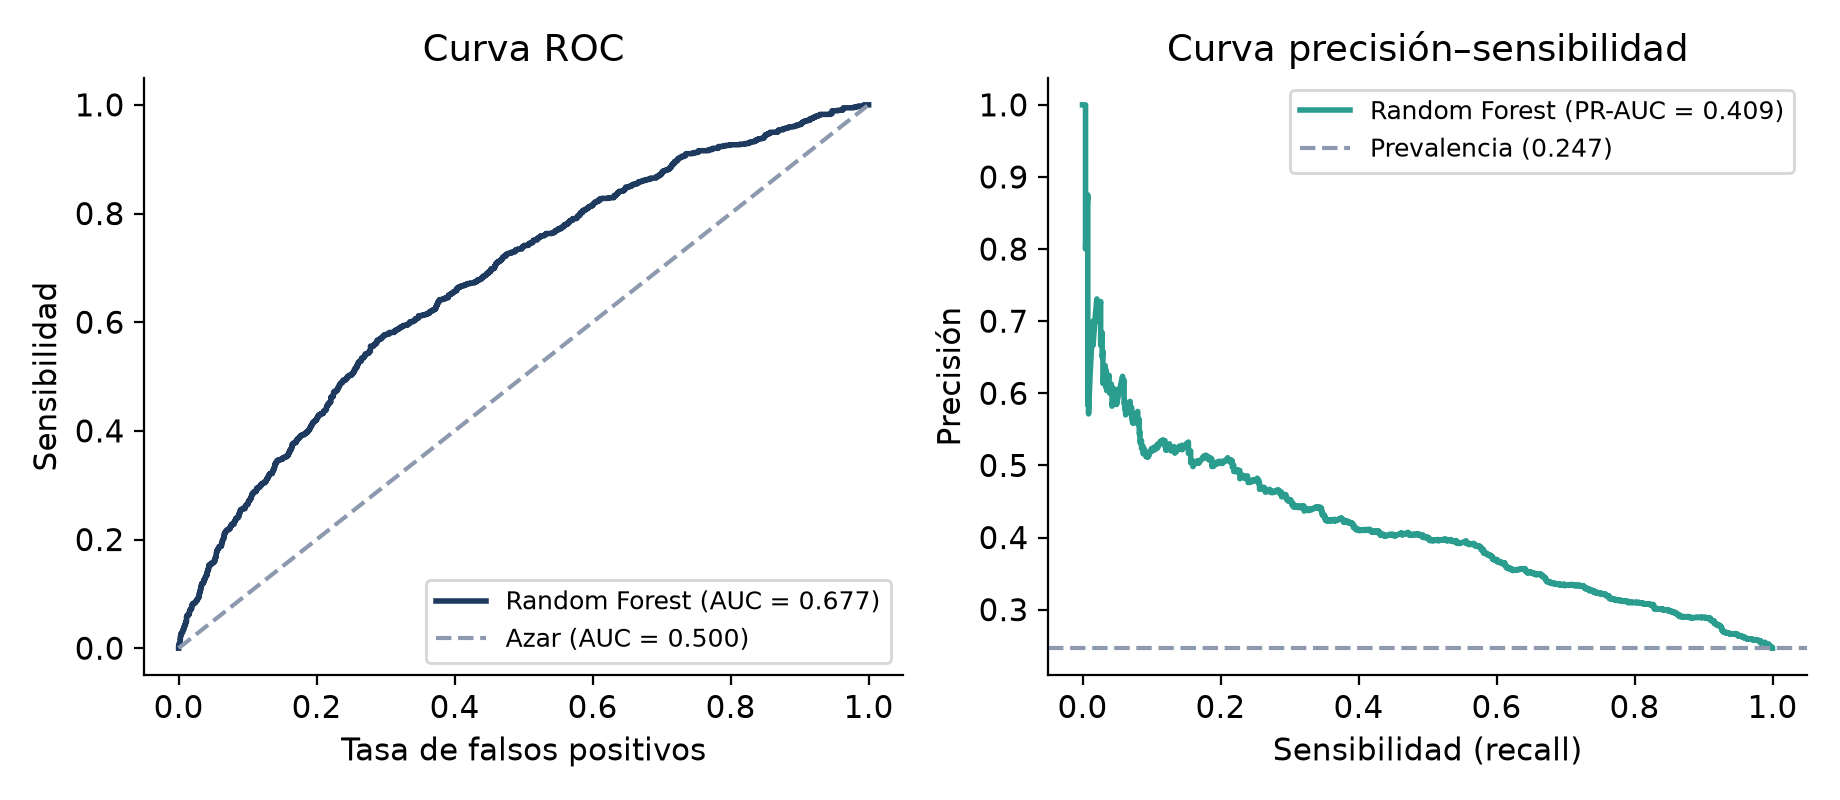
\includegraphics[width=0.95\textwidth]{figuras/curvas-roc-pr.png}
  \caption{Curvas ROC y de precisión--sensibilidad del modelo final en el conjunto de prueba. Elaboración propia.}
  \label{fig:curvas}
\end{figure}

\subsection{Desempeño en Tungurahua}
El conjunto de prueba contiene 112 registros de Tungurahua (35 con desnutrición crónica). La Tabla~\ref{tab:tung} los compara con el resto del país. Los valores puntuales son similares, pero el intervalo de Tungurahua es amplio (por ejemplo, la sensibilidad va de 0.533 a 0.833) debido al tamaño de la muestra. Por ello los resultados de Tungurahua son indicativos y no permiten afirmar que el modelo funcione mejor o peor allí que en el resto del país.

\begin{table}[H]
  \caption{Métricas del modelo en Tungurahua y en el resto del país (conjunto de prueba, umbral 0.42).}
  \label{tab:tung}
  \tablabase\small
  \begin{tabular}{|p{4.4cm}|c|c|c|}
    \hline
    \enc{Métrica} & \enc{Tungurahua} & \enc{IC 95\,\% (Tung.)} & \enc{Resto del país}\\ \hline
    Registros (casos) & 112 (35) & --- & \num{3587} (877)\\ \hline
    Sensibilidad & 0.686 & 0.533--0.833 & 0.693\\ \hline
    Especificidad & 0.571 & --- & 0.549\\ \hline
    Precisión & 0.421 & --- & 0.332\\ \hline
    F1 (clase 1) & 0.522 & 0.385--0.641 & 0.449\\ \hline
    Exactitud balanceada & 0.629 & --- & 0.621\\ \hline
    ROC-AUC & 0.667 & 0.559--0.766 & 0.678\\ \hline
    PR-AUC & 0.485 & 0.336--0.635 & 0.408\\ \hline
  \end{tabular}
\end{table}

\begin{figure}[H]
  \centering
  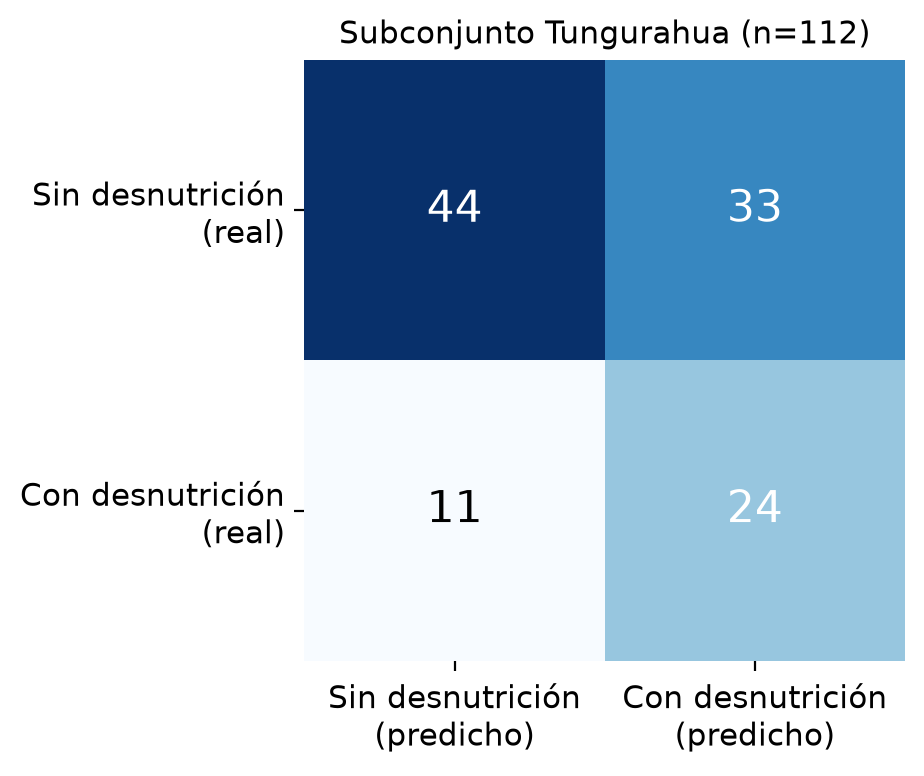
\includegraphics[width=0.5\textwidth]{figuras/matriz-confusion-tungurahua.png}
  \caption{Matriz de confusión en el subconjunto de Tungurahua del conjunto de prueba. Elaboración propia.}
  \label{fig:matriz-tung}
\end{figure}

\subsection{Sobreajuste}
El modelo se ajusta mucho mejor al entrenamiento que a la prueba (Tabla~\ref{tab:sobreajuste}): la exactitud balanceada baja de 0.819 a 0.621 y el PR-AUC de 0.815 a 0.409. Se limitó la profundidad de los árboles (20) y el tamaño de las hojas (10), pero la brecha persiste y debe considerarse al interpretar cualquier resultado.

\begin{table}[H]
  \caption{Comparación entre entrenamiento y prueba (umbral 0.42).}
  \label{tab:sobreajuste}
  \tablabase\small
  \begin{tabular}{|p{5.2cm}|c|c|}
    \hline
    \enc{Métrica} & \enc{Entrenamiento} & \enc{Prueba}\\ \hline
    Sensibilidad (clase 1) & 0.970 & 0.693\\ \hline
    Precisión (clase 1) & 0.489 & 0.335\\ \hline
    Exactitud balanceada & 0.819 & 0.621\\ \hline
    ROC-AUC & 0.932 & 0.677\\ \hline
    PR-AUC & 0.815 & 0.409\\ \hline
  \end{tabular}
\end{table}

\subsection{Comparación de los cuatro modelos por clase}

La Tabla~\ref{tab:modelos4} reporta las métricas de los cuatro modelos base en el conjunto de prueba, cada uno con su propio umbral (el que maximiza el F1 de la clase 1 por validación cruzada en el entrenamiento). Los conteos de las matrices de confusión y las curvas ROC y de precisión--sensibilidad están en el Anexo~H. El mayor PR-AUC correspondió a Random Forest (0.411), el mayor ROC-AUC a Random Forest (0.680), la mayor sensibilidad a XGBoost (0.819) y el mayor F1 a Random Forest (0.459).

La diferencia de PR-AUC entre Random Forest y Regresión logística es de 0.020; es pequeña, por lo que la elección de Random Forest debe leerse como una preferencia débil y no como una superioridad clara.

\begin{table}[H]
  \caption{Métricas de los cuatro modelos base en el conjunto de prueba, con el umbral de cada modelo (F1 máximo por validación cruzada en entrenamiento).}
  \label{tab:modelos4}
  \tablabase\scriptsize
  \begin{tabular}{|l|c|c|c|c|c|c|c|c|}
    \hline
    \enc{Modelo} & \enc{PR-AUC} & \enc{ROC-AUC} & \enc{Umbral} & \enc{Sens.} & \enc{Espec.} & \enc{Prec.} & \enc{F1} & \enc{Ex. bal.} \\ \hline
    Regresión logística & 0.391 & 0.667 & 0.470 & 0.673 & 0.574 & 0.341 & 0.453 & 0.624 \\ \hline
    Árbol de decisión & 0.263 & 0.536 & 0.050 & 0.300 & 0.773 & 0.302 & 0.301 & 0.536 \\ \hline
    Random Forest & 0.411 & 0.680 & 0.230 & 0.735 & 0.521 & 0.334 & 0.459 & 0.628 \\ \hline
    XGBoost & 0.368 & 0.648 & 0.240 & 0.819 & 0.359 & 0.295 & 0.434 & 0.589 \\ \hline
  \end{tabular}
\end{table}




\subsection{Sensibilidad al umbral de decisión}

La Figura~\ref{fig:umbral} muestra cómo cambian las métricas del modelo final al variar el umbral. Con 0.30 la sensibilidad sube a 0.959, pero la precisión baja a 0.261 y el modelo genera 3355 alertas sobre 3699 registros; con 0.42 (umbral adoptado) la sensibilidad es 0.693, la precisión 0.335 y las alertas 1887; con 0.60 la sensibilidad cae a 0.106 y la precisión sube a 0.524. No existe un umbral que alcance a la vez sensibilidad y precisión altas: la elección refleja una decisión sobre qué error se tolera más. Los valores para otros umbrales están en el Anexo~H.

\begin{figure}[H]
  \centering
  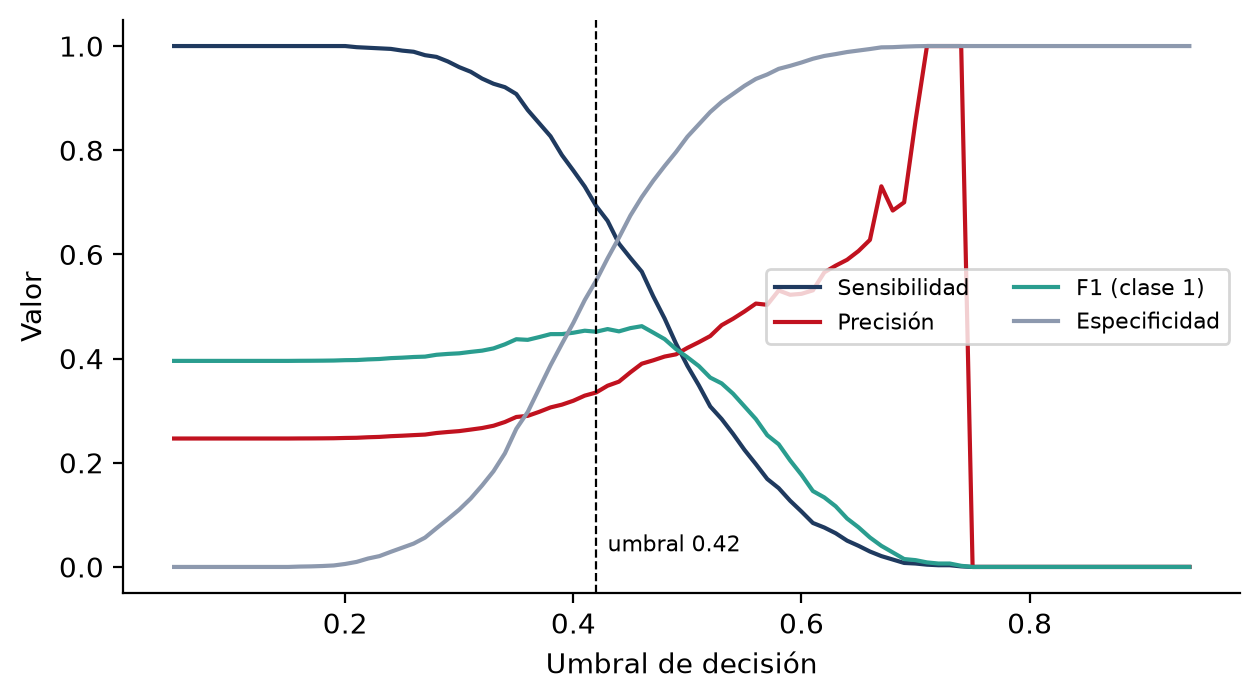
\includegraphics[width=0.75\textwidth]{figuras/anexo-umbral.png}
  \caption{Métricas del modelo final según el umbral de decisión (conjunto de prueba). Elaboración propia.}
  \label{fig:umbral}
\end{figure}



\subsection{Calibración de las probabilidades}

La calibración indica si una probabilidad predicha corresponde a la frecuencia real de casos \cite{steyerberg2019clinical}. El error de Brier del modelo final es 0.205, frente a 0.186 de un predictor que solo usa la prevalencia, es decir, es peor: las probabilidades del modelo no están calibradas. La probabilidad media predicha es 0.427 y la prevalencia observada es 0.247. En el decil más bajo la probabilidad media es 0.264 y la proporción observada 0.105; en el más alto, 0.608 y 0.505.

La probabilidad media supera la prevalencia porque el modelo se entrenó con ponderación de clases; por eso las probabilidades no deben leerse como riesgo absoluto, sino como una puntuación para ordenar casos. Esta es otra razón para no interpretar los niveles de riesgo (BAJO, MEDIO, ALTO) de la API como probabilidades reales. La curva y la distribución de probabilidades están en el Anexo~H (Figura~\ref{fig:calibracion}).



\subsection{Desempeño por subgrupos}

La Figura~\ref{fig:subgrupos} muestra la sensibilidad del modelo final (umbral 0.42) en subgrupos del conjunto de prueba nacional, con intervalos de Wilson. En el conjunto nacional, según el área, la sensibilidad va de 0.525 (Urbano; 480 casos) a 0.880 (Rural; 432 casos); según el sexo, la sensibilidad va de 0.659 (Mujer; 402 casos) a 0.720 (Hombre; 510 casos); según el grupo de edad, la sensibilidad va de 0.505 (36-59; 295 casos) a 0.892 (12-23; 259 casos).

Las diferencias son marcadas: entre Urbano y Rural los intervalos no se traslapan, y la prevalencia muestral es de 21.4\,\% y 29.7\,\% respectivamente; entre 36-59 y 12-23 los intervalos no se traslapan, y la prevalencia muestral es de 19.3\,\% y 34.0\,\% respectivamente. Con un umbral único, el modelo identifica una proporción mayor de los casos donde la prevalencia es mayor y una proporción menor donde es menor. Por eso la sensibilidad global (0.693) oculta diferencias importantes: en los subgrupos con menor prevalencia se omite cerca de la mitad de los casos. Un uso aplicado exigiría revisar el umbral por grupo. En el sexo la diferencia es menor.

El detalle, con especificidad y ROC-AUC, y los subgrupos de Tungurahua (muy pequeños, por lo que solo son indicativos) están en el Anexo~H.

\begin{figure}[H]
  \centering
  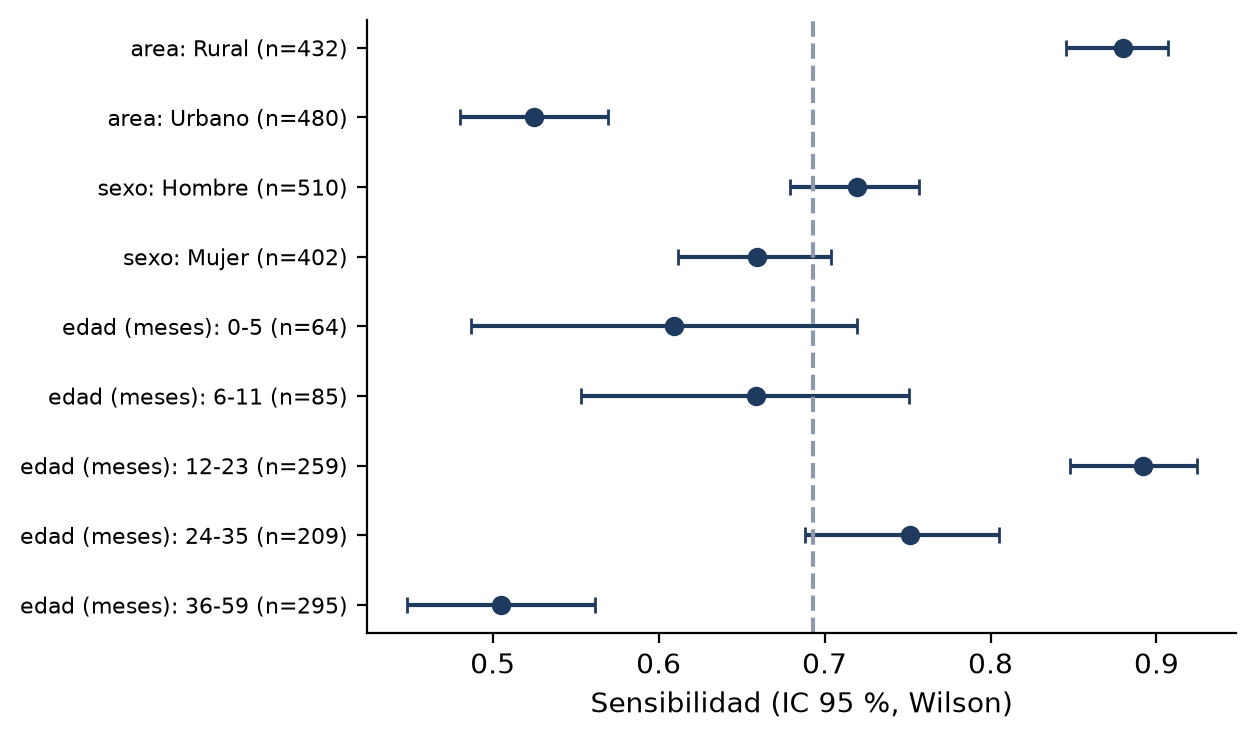
\includegraphics[width=0.8\textwidth]{figuras/anexo-subgrupos.png}
  \caption{Sensibilidad del modelo final por subgrupos en la prueba nacional (línea punteada: sensibilidad global). Elaboración propia.}
  \label{fig:subgrupos}
\end{figure}



\subsection{Análisis de errores}

La Figura~\ref{fig:errores} descompone las clasificaciones por grupo de edad. La proporción de casos omitidos (falsos negativos entre los casos reales) fue mayor en el grupo de 36-59 meses (49.5\,\%) y menor en el de 12-23 meses (10.8\,\%). La proporción de falsas alarmas (falsos positivos entre los no casos) fue mayor en 12-23 meses (75.3\,\%) y menor en 36-59 meses (29.1\,\%). Como la edad es la variable con mayor importancia del modelo, es esperable que los errores dependan de ella; un uso aplicado exigiría revisar el desempeño por edad antes de fijar un umbral único.

\begin{figure}[H]
  \centering
  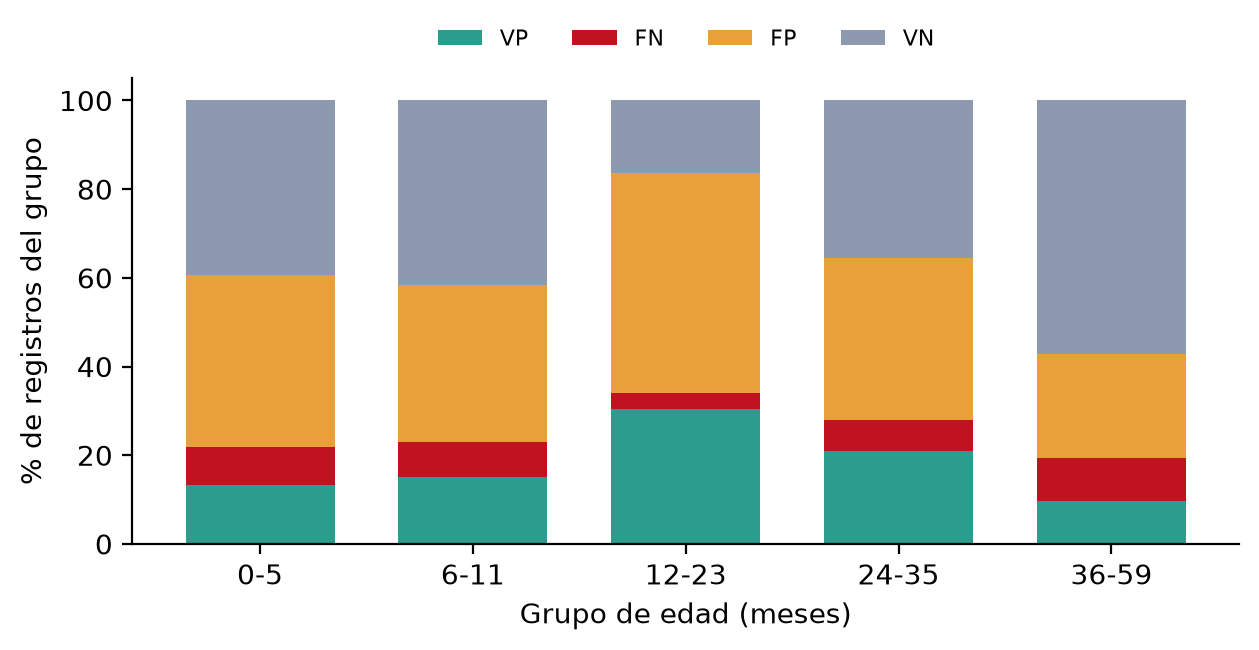
\includegraphics[width=0.75\textwidth]{figuras/anexo-errores-edad.png}
  \caption{Composición de las clasificaciones por grupo de edad (umbral 0.42). VP: verdaderos positivos; FN: falsos negativos; FP: falsos positivos; VN: verdaderos negativos. Elaboración propia.}
  \label{fig:errores}
\end{figure}



\subsection{Prueba sin las variables de diseño muestral}

Como \texttt{factor\_expansion} y \texttt{estrato} no describen al niño, se entrenó un Random Forest con los mismos hiperparámetros y la misma partición, pero sin esas dos variables. La Tabla~\ref{tab:sindiseno} muestra el resultado: el ROC-AUC pasa de 0.677 a 0.679 (diferencia de +0.002) y el PR-AUC de 0.409 a 0.408 (diferencia de -0.001). La diferencia es pequeña, por lo que el desempeño no depende de forma importante de esas dos variables y el modelo sin ellas es una alternativa más limpia. Con el umbral propio de esta versión (0.40, elegido por validación cruzada en el entrenamiento) la sensibilidad es 0.777 y la precisión 0.319. Esta prueba es un análisis de sensibilidad complementario: el modelo evaluado y desplegado sigue siendo el de 114 variables.

\begin{table}[H]
  \caption{Comparación del modelo final con una versión sin las variables de diseño muestral.}
  \label{tab:sindiseno}
  \tablabase\scriptsize
  \begin{tabular}{|p{5.6cm}|c|c|c|c|c|c|}
    \hline
    \enc{Modelo} & \enc{ROC-AUC} & \enc{PR-AUC} & \enc{Sens.} & \enc{Espec.} & \enc{Prec.} & \enc{Ex. bal.} \\ \hline
    Modelo final (con 114 variables), umbral 0.42 & 0.677 & 0.409 & 0.693 & 0.550 & 0.335 & 0.621 \\ \hline
    Sin \texttt{factor\_expansion} ni \texttt{estrato} (112 variables), umbral 0.42 & 0.679 & 0.408 & 0.717 & 0.540 & 0.338 & 0.629 \\ \hline
    Sin variables de diseño, umbral propio 0.40 & 0.679 & 0.408 & 0.777 & 0.456 & 0.319 & 0.617 \\ \hline
  \end{tabular}
\end{table}





\subsection{Importancia de variables}
La Figura~\ref{fig:importancia} muestra las 15 variables con mayor importancia (suma de sus columnas codificadas). La importancia está repartida: ninguna supera \SI{4.5}{\percent}. Encabezan la lista la edad, el nivel de instrucción de la madre y variables del recién nacido (tamaño y peso al nacer), coherentes con los determinantes descritos en la literatura \cite{nu17223608}. Sin embargo, \texttt{factor\_expansion} y \texttt{estrato}, marcadas en rojo, ocupan el segundo y cuarto lugar. Al ser variables de diseño muestral, su peso puede reflejar la estructura de la encuesta y no características del niño. Además, el peso y la talla al nacer tienen más del \SI{55}{\percent} de valores imputados, por lo que su importancia puede reflejar la ausencia del dato. La importancia de un bosque no implica causalidad.

\begin{figure}[H]
  \centering
  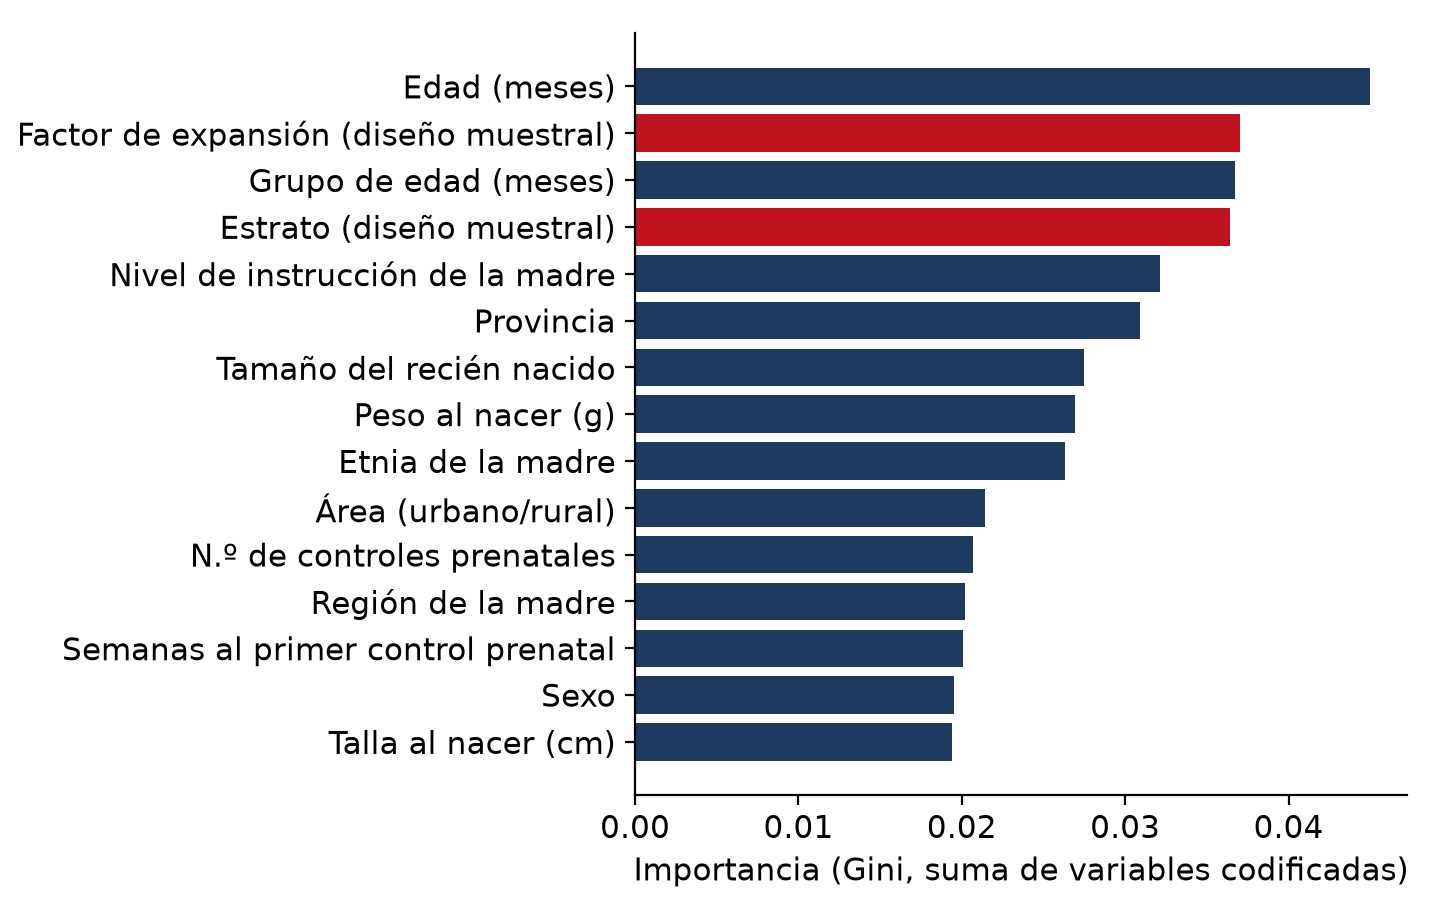
\includegraphics[width=0.85\textwidth]{figuras/importancia-variables.png}
  \caption{Importancia de las 15 variables principales del modelo final. En rojo: variables de diseño muestral. Elaboración propia.}
  \label{fig:importancia}
\end{figure}

\subsection{Comparación con la literatura}
El estudio con datos de la ENDI 2023--2024 reportó AUC de 0.62 a 0.66 para el retraso en talla en niños de 0 a 23 meses \cite{nu18142232}, y el metaanálisis con encuestas DHS, una exactitud agrupada de \SI{68.92}{\percent} \cite{ijerph22030449}. El ROC-AUC de 0.677 obtenido aquí es de magnitud similar al primero. La exactitud global de este modelo con umbral de 0.42 es de 0.585 y no es comparable con la del metaanálisis, porque el umbral se eligió para favorecer la sensibilidad. Los estudios difieren en población, variable objetivo y protocolo, por lo que la comparación es solo referencial.

\subsection{Hallazgos sobre el prototipo}
Las pruebas del sistema revelaron aspectos que deben tenerse en cuenta:
\begin{itemize}
  \item \textbf{Riesgo y clase no coincidían.} En la versión evaluada inicialmente la clase positiva se asignaba con el umbral de 0.42, pero los niveles de riesgo usaban cortes fijos de 0.50 (medio) y 0.80 (alto). En el caso CP4 la API devolvió clase 1 con probabilidad de 0.437 y riesgo BAJO; en la partición de prueba, 1050 de las 1887 clasificaciones positivas (\SI{55.6}{\percent}) figuraban como BAJO y ALTO nunca se alcanzaba (probabilidad máxima de 0.747). Se corrigió: BAJO coincide ahora con la clase 0, MEDIO va de 0.42 a 0.60 y ALTO desde 0.60 (Anexo~A, Tabla~\ref{tab:riesgo}). Los niveles ordenan los casos, pero no son probabilidades calibradas.
  \item \textbf{El resumen del tablero usaba predicciones sobre datos de entrenamiento.} En la versión evaluada inicialmente, \texttt{GET /dashboard} calculaba los ``casos'' como positivos predichos por el modelo sobre el archivo completo (\num{20510} registros, que incluye los usados para entrenar), por lo que no equivalía a la prevalencia observada (\SI{24.7}{\percent}). Se corrigió: el resumen usa el conjunto de prueba (\num{3699} registros que el modelo no vio al entrenar) y muestra juntos los casos observados (912) y los clasificados (\num{1887}), con la sensibilidad y la precisión del ámbito, que reproducen las métricas del modelo (0.693 y 0.335). En Tungurahua (112 registros) hay 35 casos observados y 57 clasificados, con una sensibilidad de 0.686 que es inestable por el tamaño de la muestra.
  \item \textbf{Imputación previa a la partición y muy alta en variables clave.} Los faltantes se imputaron antes de dividir los datos, y variables muy importantes del modelo tienen más de la mitad de sus valores imputados (peso y talla al nacer). Como un valor imputado coincide con la mediana, el modelo puede estar usando el hecho de que el dato faltaba y no el valor real; su importancia debe interpretarse con esa reserva.
  \item \textbf{El formulario de clasificación individual solo es ilustrativo.} La versión inicial del tablero pedía 8 datos y completaba las otras 106 variables con el valor 0 (y las categóricas con códigos numéricos que el modelo no vio en el entrenamiento): en 270 combinaciones la probabilidad varió solo de 0.436 a 0.512 y todas quedaron clasificadas con desnutrición. Se corrigió: el formulario envía las 114 variables (las no informadas como nulas, que el \textit{Pipeline} imputa) con las categorías válidas y la edad agrupada correcta. Aun así, en 512 combinaciones de prueba la probabilidad varió solo de 0.375 a 0.515 y el \SI{85.5}{\percent} quedó clasificado con desnutrición (CP15), porque el resto de las variables se imputa. Por eso la pantalla lo declara de uso ilustrativo y remite a la clasificación por archivo.
  \item \textbf{Carga de archivos Excel.} La pantalla mencionaba archivos \texttt{.xlsx}, pero en la versión evaluada inicialmente el servicio solo leía CSV y un Excel enviado a la API producía una excepción no controlada (CP14). Se corrigió: la API lee \texttt{.xlsx} y devuelve el mismo resultado que con el CSV equivalente, y ante un Excel dañado, un \texttt{.xls}, un archivo vacío o sin registros responde con un mensaje de error en lugar de una excepción. El tablero acepta solo CSV y muestra un mensaje claro con las columnas faltantes (CP16).
  \item \textbf{Página de métricas del tablero.} Leía los nombres de métricas de la versión anterior (\texttt{accuracy}, \texttt{recall}\ldots) y con la API v2 habría mostrado valores no numéricos; se actualizó para mostrar la sensibilidad, la precisión, el F1, la exactitud balanceada, el ROC-AUC y el PR-AUC de \texttt{metricas\_v2.json}.
  \item \textbf{Lenguaje de la interfaz.} La interfaz inicial usaba términos clínicos (``Sistema ML Clínico'', ``Predicción Clínica'', ``alto grado de confianza clínica'') y mencionaba XGBoost, aunque el modelo activo es Random Forest. Se corrigió: todas las pantallas muestran un aviso de herramienta académica exploratoria, se retiró el lenguaje clínico, el nombre del modelo se lee de la API y el resumen de indicadores aclara que las cifras son del conjunto de prueba y no la prevalencia poblacional (Anexo~B).
\end{itemize}

\subsection{Síntesis de resultados}
La Tabla~\ref{tab:cumplimiento} indica el estado de cada requerimiento según la evidencia de este capítulo.

\begin{table}[H]
  \caption{Cumplimiento de los requerimientos.}
  \label{tab:cumplimiento}
  \tablabase\footnotesize
  \begin{tabular}{|c|c|p{9.4cm}|}
    \hline
    \enc{ID} & \enc{Estado} & \enc{Evidencia}\\ \hline
    RF1 & Cumple & Pipeline con preprocesamiento ajustado solo en entrenamiento; semilla 42\\ \hline
    RF2 & Cumple & Tabla~\ref{tab:experimento}, Tabla~\ref{tab:metricas} y Figura~\ref{fig:comparacion}\\ \hline
    RF3 & Cumple & CP4 a CP7 (Anexo~C)\\ \hline
    RF4 & Cumple & CP8: un CSV de 50 registros devuelve 50 filas; CP14: un Excel de 50 registros devuelve 50 filas y los archivos inválidos reciben un mensaje de error\\ \hline
    RF5 & Cumple & CP11: métricas idénticas a \texttt{metricas\_v2.json}\\ \hline
    RF6 & Cumple & CP9, CP10 y CP12: el resumen usa el conjunto de prueba y reproduce las métricas de \texttt{metricas\_v2.json}\\ \hline
    RF7 & Cumple & CP13\\ \hline
    RF8 & Cumple & Prueba de contrato de versión del modelo\\ \hline
    RNF1 & Cumple & CP5, CP6 y CP7: HTTP 400 en los tres casos\\ \hline
    RNF2 & Cumple & Mediana de 29 ms en 100 solicitudes (local)\\ \hline
    RNF3 & Cumple & CP1 (\texttt{GET /health}). No se midió disponibilidad en el tiempo\\ \hline
    RNF4 & No cumple & La API no implementa autenticación; el CORS está abierto\\ \hline
    RNF5 & Cumple & Semilla y versiones fijadas en \texttt{requirements.txt}\\ \hline
    RNF6 & Cumple & Módulos separados y 21 pruebas automáticas aprobadas\\ \hline
    RNF7 & Cumple & Aviso académico visible en todas las pantallas y lenguaje clínico retirado (Anexo~B)\\ \hline
  \end{tabular}
\end{table}

En síntesis, el prototipo cumple 14 de los 15 requerimientos y 1 no se cumple. El modelo tiene un desempeño moderado (ROC-AUC de 0.677), sobreajuste medido y ninguna validación externa; sus productos son una API funcional con datos completos y un tablero de consulta cuyo formulario individual solo es ilustrativo. Quedan pendientes la autenticación y la validación con una fuente independiente.

\section{Cronograma y Presupuesto}
\subsection{Cronograma de Ejecución}
La Tabla~\ref{tab:cronograma} presenta las actividades ejecutadas. \pend{verificar las fechas reales de cada actividad; las anteriores a septiembre provienen de la versión previa del documento}

\begingroup
\footnotesize\setlength{\tabcolsep}{4pt}\arrayrulecolor{black!55}\renewcommand{\arraystretch}{1.1}
\begin{longtable}{|c|p{5.2cm}|c|c|p{2.8cm}|}
  \caption{Cronograma de actividades del proyecto.}
  \label{tab:cronograma}\\ \hline
  \enc{N.º} & \enc{Actividad} & \enc{Inicio} & \enc{Fin} & \enc{Resultado}\\ \hline
  \endfirsthead
  \tablacont{5}\hline
  \enc{N.º} & \enc{Actividad} & \enc{Inicio} & \enc{Fin} & \enc{Resultado}\\ \hline
  \endhead
  \hline\endfoot
  1 & Revisión bibliográfica y definición del problema & 04/05/2026 & 08/05/2026 & Marco conceptual\\ \hline
  2 & Recopilación y revisión de los datos ENSANUT (y exploración de ENDI) & 09/05/2026 & 12/05/2026 & Datos brutos\\ \hline
  3 & Auditoría técnica y análisis exploratorio & 13/05/2026 & 20/05/2026 & Diagnóstico de calidad\\ \hline
  4 & Limpieza y preparación de variables & 21/05/2026 & 29/05/2026 & Dataset preparado\\ \hline
  5 & Entrenamiento inicial de modelos (v1) & 30/05/2026 & 06/06/2026 & Modelos base\\ \hline
  6 & Optimización de hiperparámetros (v1) & 07/06/2026 & 13/06/2026 & Modelo optimizado\\ \hline
  7 & Evaluación y selección del modelo (v1) & 14/06/2026 & 18/06/2026 & Modelo seleccionado\\ \hline
  8 & Serialización del modelo & 19/06/2026 & 21/06/2026 & Archivo \texttt{.joblib}\\ \hline
  9 & Desarrollo de la API REST & 22/06/2026 & 30/06/2026 & Servicios implementados\\ \hline
  10 & Pruebas funcionales de la API & 01/07/2026 & 04/07/2026 & API verificada\\ \hline
  11 & Redacción de la primera versión del documento & 05/07/2026 & 13/07/2026 & Documento inicial\\ \hline
  12 & Revisión del pipeline y reentrenamiento (v2) & 12/09/2026 & 13/09/2026 & Modelo v2 y métricas\\ \hline
  13 & Integración de v2 en la API y pruebas de contrato & 13/09/2026 & 13/09/2026 & API con v2\\ \hline
  14 & Reestructuración del documento según observaciones & 14/09/2026 & 20/09/2026 & Documento corregido\\ \hline
\end{longtable}
\endgroup

\subsection{Presupuesto}
El desarrollo usó software libre y un equipo del investigador. La Tabla~\ref{tab:presupuesto} presenta el presupuesto estimado. \pend{confirmar los montos reales de conectividad, energía, servicios en la nube e impresión}

\begin{table}[H]
  \caption{Presupuesto estimado del proyecto.}
  \label{tab:presupuesto}
  \tablabase\footnotesize
  \begin{tabular}{|p{4.2cm}|c|c|r|}
    \hline
    \enc{Recurso} & \enc{Cantidad} & \enc{Costo unitario (USD)} & \enc{Subtotal (USD)}\\ \hline
    Equipo informático (propio) & 1 & 0.00 & 0.00\\ \hline
    Software libre (Python, FastAPI, scikit-learn, React) & 1 & 0.00 & 0.00\\ \hline
    Conexión a internet & 2 meses & 25.00 & 50.00\\ \hline
    Energía eléctrica & 2 meses & 15.00 & 30.00\\ \hline
    Servicios en la nube (pruebas de despliegue) & 1 & 20.00 & 20.00\\ \hline
    Impresión y encuadernación & 1 & 25.00 & 25.00\\ \hline
    Contingencias & 1 & 25.00 & 25.00\\ \hline
    \textbf{Total estimado} & & & \textbf{150.00}\\ \hline
  \end{tabular}
\end{table}
